%! Author = rikpe
%! Date = 24/04/2021

\section{Ontwikkeling en uitvoering (DevOps)}\label{sec:ontwikkeling-en-uitvoering-(devops)}
%Leer uitkomst 5 - Development and Operations (DevOps) Je zet een omgeving en teamprocessen op die een volledig
%geautomatiseerde softwarelevenscyclus ondersteunen, terwijl je een hoge kwaliteit, hoge beschikbaarheid, snelle
%levering en korte releasetijden garandeert.
%Verdere verduidelijking Wijzigingen in de software worden ingevoerd in een goed gedefinieerd proces volgens change
%management en release procedures.
%U ontwikkelt bedrijfssoftware met behulp van CI/CD-pijplijnen.
%I/CD staat voor continuous integration en continuous delivery en/of continuous deployment.
%De CI/CD-pijplijn voert geautomatiseerde tests uit, waaronder unit tests, component tests, integratietests en
%gebruikersacceptatietests.
%Daarnaast wordt een rapport over code coverage en statische code kwaliteit gegenereerd.
%De CI/CD pipeline, testomgeving en deployment worden gecontaineriseerd.
%De implementatie van (micro)services zal worden opgeschaald wanneer nodig met behulp van container orchestration.


%Wat wil ik leren / %Wat moet ik doen om dit te kunnen bereiken? / %Welke middelen heb ik hiervoor nodig?
Voor dit leerdoel wil ik leren hoe ik een automatische test pipeline (CI/CD) opzet door middel van Github actions.
Hierbij wordt een automatische test flow opgezet die valideert of een build is geslaagd.
Wanneer deze build en de daarbij horende testen succesvol zijn uitgevoerd, wordt de image naar een production environment gestuurd waarna
de software vervolgens live wordt gezet en gebruikt kan worden door de klant.
Dit gebeurt door middel van een Kubernetes cluster.
Ook ga ik tooling gebruiken voor het bijhouden van de te ontwikkelen functionaliteiten.
Hierbij wordt in het groepsproject Devops gebruikt en voor mijn individueel project ga ik hier het Github issue-board voor gebruiken.

%Hoe ga ik success meetbaar maken?
Dit leerdoel is meetbaar te maken door de leraar proactief te informeren over hoe het ontwikkelproces zich vordert.
Ook ga ik mijn Github actions CI/CD pipeline laten zien waar de code wordt gecontroleerd op geslaagde testen en kwaliteit.
De kwaliteit van de code word getest met SonarCloud.


\subsection{Ontwikkel process}
\subsubsection{Github actions}
\paragraph{Evaluatie: 05-04-2021}
Voor het toepassen van de CI/CD pipeline verwacht ik niet enorm veel werk.
Dit is mede omdat ik in semester drie maar ook in vier hier al mee heb gewerkt en dit al eerder heb geïmplementeerd.
Daarom zie ik tijdens dit semester meer mogelijkheden voor verbetering van dit proces.
Voor mijn CI/CD module heb ik gekozen voor het toepassen van Github actions.
Mijn pipeline controleert op zowel geslaagde testen als op de code kwaliteit.
Elke microservice binnen mijn applicatie heeft zijn eigen pipeline met checks.
Hieronder is de uitwerking van een van deze pipelines voor de microservice "Article".
Hierbij is te zien dat deze pipeline verschillende checks heeft waar hij doorheen loopt.\\

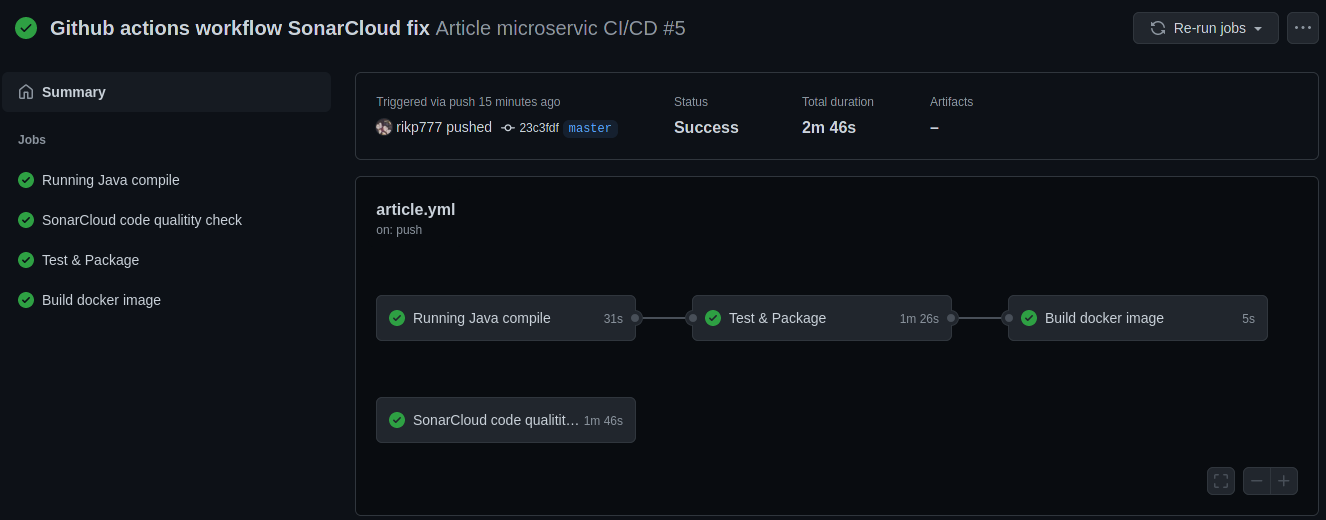
\includegraphics[width=\textwidth]{Article_Service_CI_CD_Pipeline.png}\label{fig:figure}


Via SonarCloud wordt de code gecontroleerd op kwaliteit en wordt aangekaart welke verbeteringen er kunnen plaatsvinden.\\

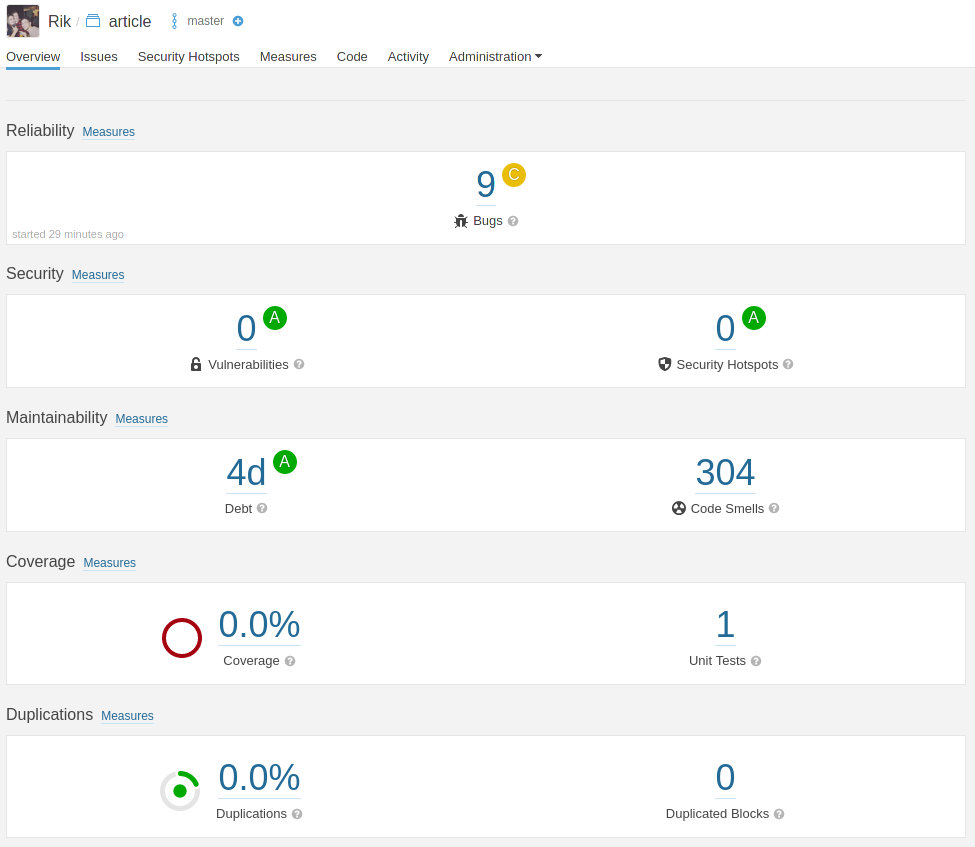
\includegraphics[width=\textwidth]{Article_Code_Quality_SonarCloud.png}\label{fig:figure2}


Omdat ik een gehele CI/CD pipeline heb geïmplementeerd voor mijn individueel project en mede door de uitwerking hierboven oriënteer ik mijzelf als:
\par\vspace{10pt}\textbf{\uppercase{"Proficient"}}.\\

Ik zou de beoordeling kunnen verbeteren naar een 'outstanding' door middel van het implementeren van een kubernetes cluster.

\subsection{Eind beoordeling / reflectie}
%Omdat ik een gehele CI/CD pipeline heb geimplementeeerd voor mijn individuele project door de uitwerking hierboven oriënteer ik mijzelf als proficient:
%\par\vspace{10pt}\textbf{\uppercase{"Proficient"}}\\

